\chapter{Goals and Use Cases}
\label{ch:Goals and Use Cases}


\section{Goals}
In this section, we describe the goals of the project.






\paragraph{}
The structure of the project consists of a component that manages and orchestrates the network (Management and orchestration,MANO) and Network Service Descriptor (NSD) that specify the network service to be created and it is a collection of configuration documents which determines how the network service is comprised in terms of Virtual Network Functions (VNFs).
 



\paragraph{}
The main goal of the project is to build three work packages:

\begin{enumerate}
	\item Service Descriptor Translator(SDT) : SDT  translates Network Service descriptor (NSD) of one MANO framework (mano1) to another MANO framework (mano2). In the structure given, translator is required if  mano2 needs to deploy the services described by NSD of mano1.
	\item Service Descriptor Splitter(SDS) : In order to deploy VNFs over different Point of presence (POPs), splitter is required.
	\item MANO scalability support : Adaptor is necessary if more than one instance of MANO framework is needed, i.e,  adaptor allows interaction between different instances of MANO frameworks. It also exposes the underlying MANOs service instantiation interfaces and retrieves monitoring information about the service status.
\end{enumerate}

\begin{figure}
	\centering
	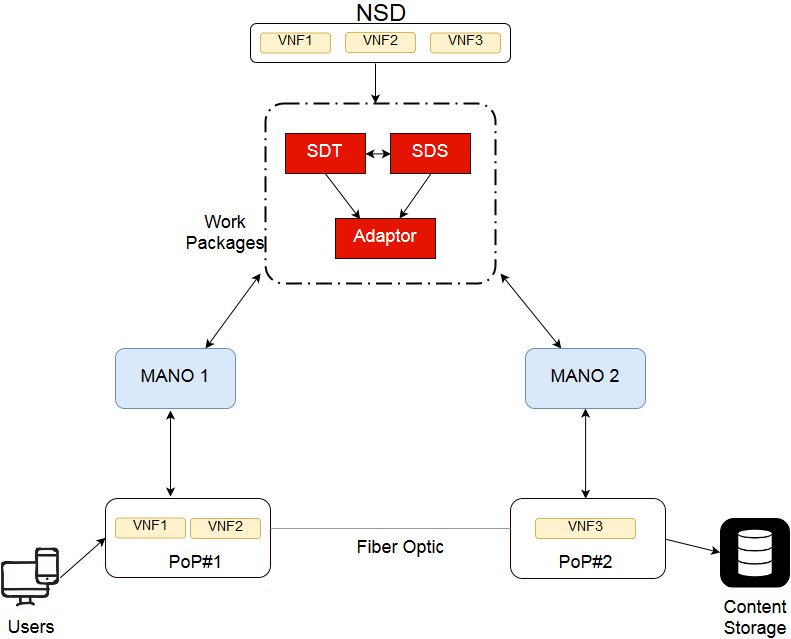
\includegraphics[width=0.7\linewidth]{figures/Structure_Updated1}
	\caption{This figure visualizes the structure of the project. }
	\label{fig:structureupdated1}
\end{figure}


\newpage
\section{Use Cases}

\subsection{Cross MANO Framework interaction}
\paragraph{}

As a matter of fact , the MANO frameworks used by every network service provider varies from one another. 
Network service Descriptor translation enables the deployment of network services that is in accordance with the intended framework

For instance : If an operator uses Sonata framework and another operator uses OSM operator, the NSD schemas for both the frameworks will be different. Using the solutions of translation and splitting, network services can be deployed and orchestrated across MANO implementations.

\subsection{Hierarchical orchestration}
\paragraph{}
By implementing MANO adaptor , dynamic instantiation and inter-operability between different MANO frameworks 
can be achieved. As a result of this goal, operators will be able to scale up and scale down the resources as and when required. Also the operator will be able to handle the resources in an efficient manner. 
When there is a high demand for network service , the operator can explore options to include additional MANO instances to mitigate the traffic load on a single MANO instance.The resources can be provisioned based on the amount of requests. This helps the operator in extending profitability. 























